\documentclass{standalone}
\usepackage{tikz}
\usetikzlibrary{matrix,backgrounds}

\begin{document}
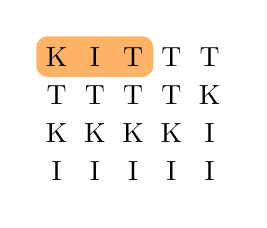
\begin{tikzpicture}
  \matrix (m) [matrix of nodes,
                nodes={minimum size=5mm, anchor=center, inner sep=0pt},
                row sep=-\pgflinewidth,
                column sep=-\pgflinewidth]
  {
    K & I & T & T & T \\ 
    T & T & T & T & K \\ 
    K & K & K & K & I \\ 
    I & I & I & I & I \\ 
  };
  \begin{scope}[on background layer]
    \fill[orange, opacity=0.6, rounded corners]
      (m-1-1.north west) --
      (m-1-3.north east) --
      (m-1-3.south east) --
      (m-1-1.south west) --
      cycle;
  \end{scope}
\end{tikzpicture}
\end{document}

